\documentclass{article}\usepackage[]{graphicx}\usepackage[]{color}
%% maxwidth is the original width if it is less than linewidth
%% otherwise use linewidth (to make sure the graphics do not exceed the margin)
\makeatletter
\def\maxwidth{ %
  \ifdim\Gin@nat@width>\linewidth
    \linewidth
  \else
    \Gin@nat@width
  \fi
}
\makeatother

\definecolor{fgcolor}{rgb}{0.345, 0.345, 0.345}
\newcommand{\hlnum}[1]{\textcolor[rgb]{0.686,0.059,0.569}{#1}}%
\newcommand{\hlstr}[1]{\textcolor[rgb]{0.192,0.494,0.8}{#1}}%
\newcommand{\hlcom}[1]{\textcolor[rgb]{0.678,0.584,0.686}{\textit{#1}}}%
\newcommand{\hlopt}[1]{\textcolor[rgb]{0,0,0}{#1}}%
\newcommand{\hlstd}[1]{\textcolor[rgb]{0.345,0.345,0.345}{#1}}%
\newcommand{\hlkwa}[1]{\textcolor[rgb]{0.161,0.373,0.58}{\textbf{#1}}}%
\newcommand{\hlkwb}[1]{\textcolor[rgb]{0.69,0.353,0.396}{#1}}%
\newcommand{\hlkwc}[1]{\textcolor[rgb]{0.333,0.667,0.333}{#1}}%
\newcommand{\hlkwd}[1]{\textcolor[rgb]{0.737,0.353,0.396}{\textbf{#1}}}%

\usepackage{framed}
\makeatletter
\newenvironment{kframe}{%
 \def\at@end@of@kframe{}%
 \ifinner\ifhmode%
  \def\at@end@of@kframe{\end{minipage}}%
  \begin{minipage}{\columnwidth}%
 \fi\fi%
 \def\FrameCommand##1{\hskip\@totalleftmargin \hskip-\fboxsep
 \colorbox{shadecolor}{##1}\hskip-\fboxsep
     % There is no \\@totalrightmargin, so:
     \hskip-\linewidth \hskip-\@totalleftmargin \hskip\columnwidth}%
 \MakeFramed {\advance\hsize-\width
   \@totalleftmargin\z@ \linewidth\hsize
   \@setminipage}}%
 {\par\unskip\endMakeFramed%
 \at@end@of@kframe}
\makeatother

\definecolor{shadecolor}{rgb}{.97, .97, .97}
\definecolor{messagecolor}{rgb}{0, 0, 0}
\definecolor{warningcolor}{rgb}{1, 0, 1}
\definecolor{errorcolor}{rgb}{1, 0, 0}
\newenvironment{knitrout}{}{} % an empty environment to be redefined in TeX

\usepackage{alltt}
\IfFileExists{upquote.sty}{\usepackage{upquote}}{}
\begin{document}

\begin{knitrout}
\definecolor{shadecolor}{rgb}{0.969, 0.969, 0.969}\color{fgcolor}\begin{kframe}
\begin{alltt}
\hlcom{# GUIA 10}

\hlstd{A} \hlkwb{<-} \hlkwd{c}\hlstd{(}\hlnum{100}\hlstd{,}\hlnum{96}\hlstd{,}\hlnum{92}\hlstd{,}\hlnum{96}\hlstd{,}\hlnum{92}\hlstd{); A}
\end{alltt}
\begin{verbatim}
## [1] 100  96  92  96  92
\end{verbatim}
\begin{alltt}
\hlstd{B} \hlkwb{<-} \hlkwd{c}\hlstd{(}\hlnum{76}\hlstd{,}\hlnum{80}\hlstd{,}\hlnum{75}\hlstd{,}\hlnum{84}\hlstd{,}\hlnum{82}\hlstd{); B}
\end{alltt}
\begin{verbatim}
## [1] 76 80 75 84 82
\end{verbatim}
\begin{alltt}
\hlstd{C} \hlkwb{<-} \hlkwd{c}\hlstd{(}\hlnum{108}\hlstd{,}\hlnum{100}\hlstd{,}\hlnum{96}\hlstd{,}\hlnum{98}\hlstd{,}\hlnum{100}\hlstd{); C}
\end{alltt}
\begin{verbatim}
## [1] 108 100  96  98 100
\end{verbatim}
\begin{alltt}
\hlstd{Baterias} \hlkwb{<-} \hlkwd{data.frame}\hlstd{(}\hlkwc{procesoA}\hlstd{=A,} \hlkwc{procesoB}\hlstd{=B,} \hlkwc{procesoC}\hlstd{=C); Baterias}
\end{alltt}
\begin{verbatim}
##   procesoA procesoB procesoC
## 1      100       76      108
## 2       96       80      100
## 3       92       75       96
## 4       96       84       98
## 5       92       82      100
\end{verbatim}
\begin{alltt}
\hlkwd{fix}\hlstd{(Baterias)}
\hlkwd{write.table}\hlstd{(Baterias,} \hlkwc{file}\hlstd{=}\hlstr{"Baterias.txt"}\hlstd{,} \hlkwc{append}\hlstd{=}\hlnum{FALSE}\hlstd{,} \hlkwc{quote}\hlstd{=}\hlnum{TRUE}\hlstd{,} \hlkwc{sep}\hlstd{=}\hlstr{" "}\hlstd{,} \hlkwc{na}\hlstd{=}\hlstr{"NA"}\hlstd{,}\hlkwc{col.names}\hlstd{=}\hlnum{TRUE}\hlstd{)}
\hlkwd{ls}\hlstd{();} \hlkwd{rm}\hlstd{(}\hlkwc{list}\hlstd{=}\hlkwd{ls}\hlstd{(}\hlkwc{all}\hlstd{=}\hlnum{TRUE}\hlstd{));} \hlkwd{ls}\hlstd{()}
\end{alltt}
\begin{verbatim}
## [1] "A"        "B"        "Baterias" "C"
## character(0)
\end{verbatim}
\begin{alltt}
\hlstd{Baterias} \hlkwb{<-} \hlkwd{read.table}\hlstd{(}\hlstr{"Baterias.txt"}\hlstd{,} \hlkwc{header}\hlstd{=}\hlnum{TRUE}\hlstd{); Baterias}
\end{alltt}
\begin{verbatim}
##   procesoA procesoB procesoC
## 1      100       76      108
## 2       96       80      100
## 3       92       75       96
## 4       96       84       98
## 5       92       82      100
\end{verbatim}
\begin{alltt}
\hlkwd{attach}\hlstd{(Baterias,} \hlkwc{pos}\hlstd{=}\hlnum{2}\hlstd{)}
\hlkwd{search}\hlstd{()}
\end{alltt}
\begin{verbatim}
##  [1] ".GlobalEnv"        "Baterias"          "package:knitr"    
##  [4] "package:stats"     "package:graphics"  "package:grDevices"
##  [7] "package:utils"     "package:datasets"  "package:methods"  
## [10] "Autoloads"         "package:base"
\end{verbatim}
\begin{alltt}
\hlkwd{stripchart}\hlstd{(Baterias,} \hlkwc{main}\hlstd{=}\hlstr{"Gr�fico de puntos para los tres procesos"}\hlstd{,} \hlkwc{method} \hlstd{=} \hlstr{"stack"}\hlstd{,} \hlkwc{vertical} \hlstd{=}
\hlnum{FALSE}\hlstd{,} \hlkwc{col}\hlstd{=}\hlstr{"blue"}\hlstd{,} \hlkwc{pch}\hlstd{=}\hlnum{1}\hlstd{,} \hlkwc{xlab}\hlstd{=}\hlstr{"Duraci�n (semanas)"}\hlstd{,} \hlkwc{ylab}\hlstd{=}\hlstr{"Proceso"}\hlstd{)}
\end{alltt}
\end{kframe}
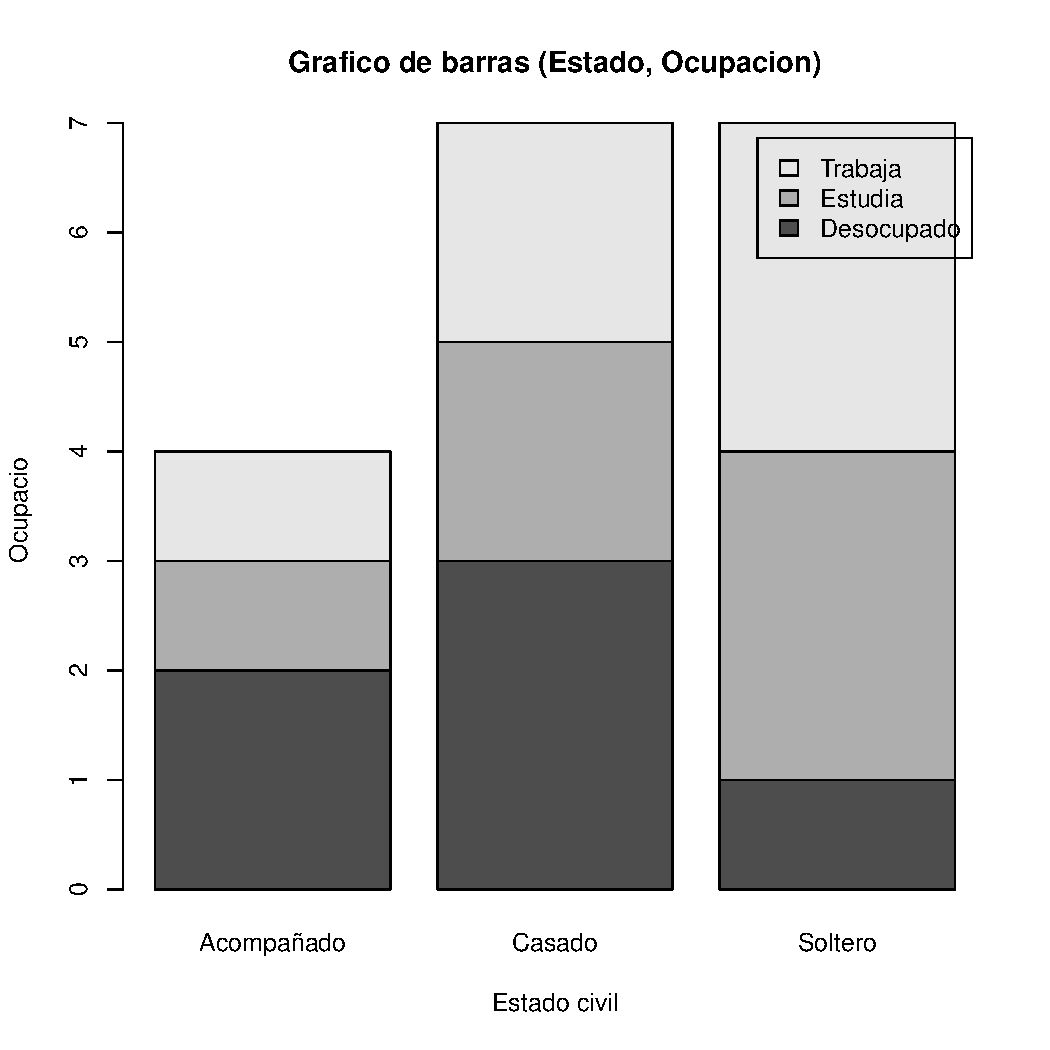
\includegraphics[width=\maxwidth]{figure/unnamed-chunk-1-1} 
\begin{kframe}\begin{alltt}
\hlkwd{summary}\hlstd{(Baterias)}
\end{alltt}
\begin{verbatim}
##     procesoA        procesoB       procesoC    
##  Min.   : 92.0   Min.   :75.0   Min.   : 96.0  
##  1st Qu.: 92.0   1st Qu.:76.0   1st Qu.: 98.0  
##  Median : 96.0   Median :80.0   Median :100.0  
##  Mean   : 95.2   Mean   :79.4   Mean   :100.4  
##  3rd Qu.: 96.0   3rd Qu.:82.0   3rd Qu.:100.0  
##  Max.   :100.0   Max.   :84.0   Max.   :108.0
\end{verbatim}
\begin{alltt}
\hlcom{# Horizontal}
\hlkwd{boxplot}\hlstd{(Baterias,} \hlkwc{width}\hlstd{=}\hlkwa{NULL}\hlstd{,} \hlkwc{varwidth}\hlstd{=}\hlnum{TRUE}\hlstd{, names,} \hlkwc{add}\hlstd{=} \hlnum{FALSE}\hlstd{,} \hlkwc{horizontal} \hlstd{=} \hlnum{TRUE}\hlstd{,}
\hlkwc{main}\hlstd{=}\hlstr{"Gr�fico de caja por proceso"}\hlstd{,} \hlkwc{border}\hlstd{=}\hlkwd{par}\hlstd{(}\hlstr{"fg"}\hlstd{),} \hlkwc{col}\hlstd{=}\hlkwd{c}\hlstd{(}\hlstr{"yellow"}\hlstd{,} \hlstr{"cyan"}\hlstd{,} \hlstr{"red"}\hlstd{),} \hlkwc{xlab} \hlstd{=}
\hlstr{"Duraci�n (semanas)"}\hlstd{,} \hlkwc{ylab}\hlstd{=}\hlstr{"Proceso"}\hlstd{)}
\end{alltt}
\end{kframe}
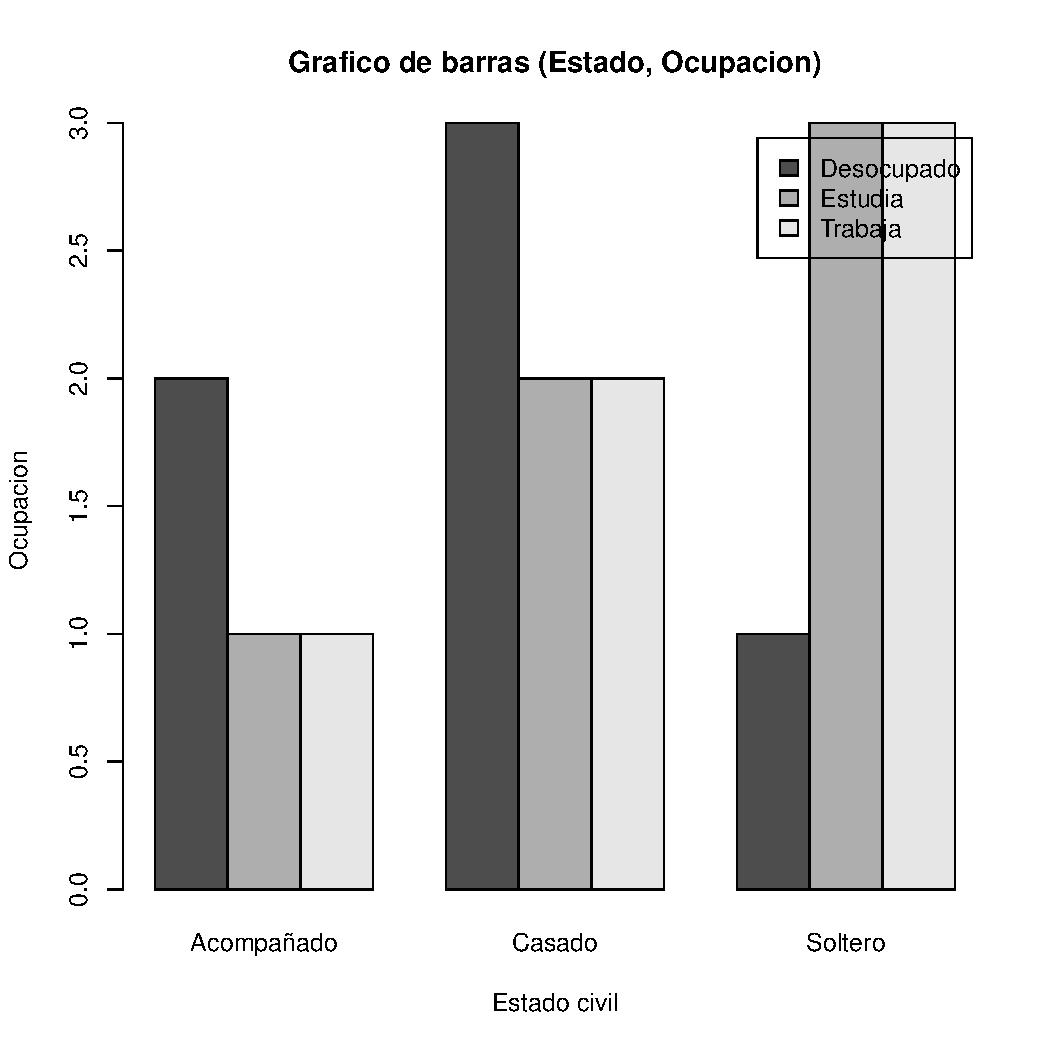
\includegraphics[width=\maxwidth]{figure/unnamed-chunk-1-2} 
\begin{kframe}\begin{alltt}
\hlcom{# Vertical}
\hlkwd{boxplot}\hlstd{(Baterias,} \hlkwc{width}\hlstd{=}\hlkwa{NULL}\hlstd{,} \hlkwc{varwidth}\hlstd{=}\hlnum{TRUE}\hlstd{, names,} \hlkwc{add}\hlstd{=} \hlnum{FALSE}\hlstd{,} \hlkwc{horizontal} \hlstd{=} \hlnum{FALSE}\hlstd{,}
\hlkwc{main}\hlstd{=}\hlstr{"Gr�fico de caja por proceso"}\hlstd{,} \hlkwc{border}\hlstd{=}\hlkwd{par}\hlstd{(}\hlstr{"fg"}\hlstd{),} \hlkwc{col}\hlstd{=}\hlkwd{c}\hlstd{(}\hlstr{"yellow"}\hlstd{,} \hlstr{"cyan"}\hlstd{,} \hlstr{"red"}\hlstd{),} \hlkwc{xlab} \hlstd{=}
\hlstr{"Duraci�n (semanas)"}\hlstd{,} \hlkwc{ylab}\hlstd{=}\hlstr{"Proceso"}\hlstd{)}
\end{alltt}
\end{kframe}
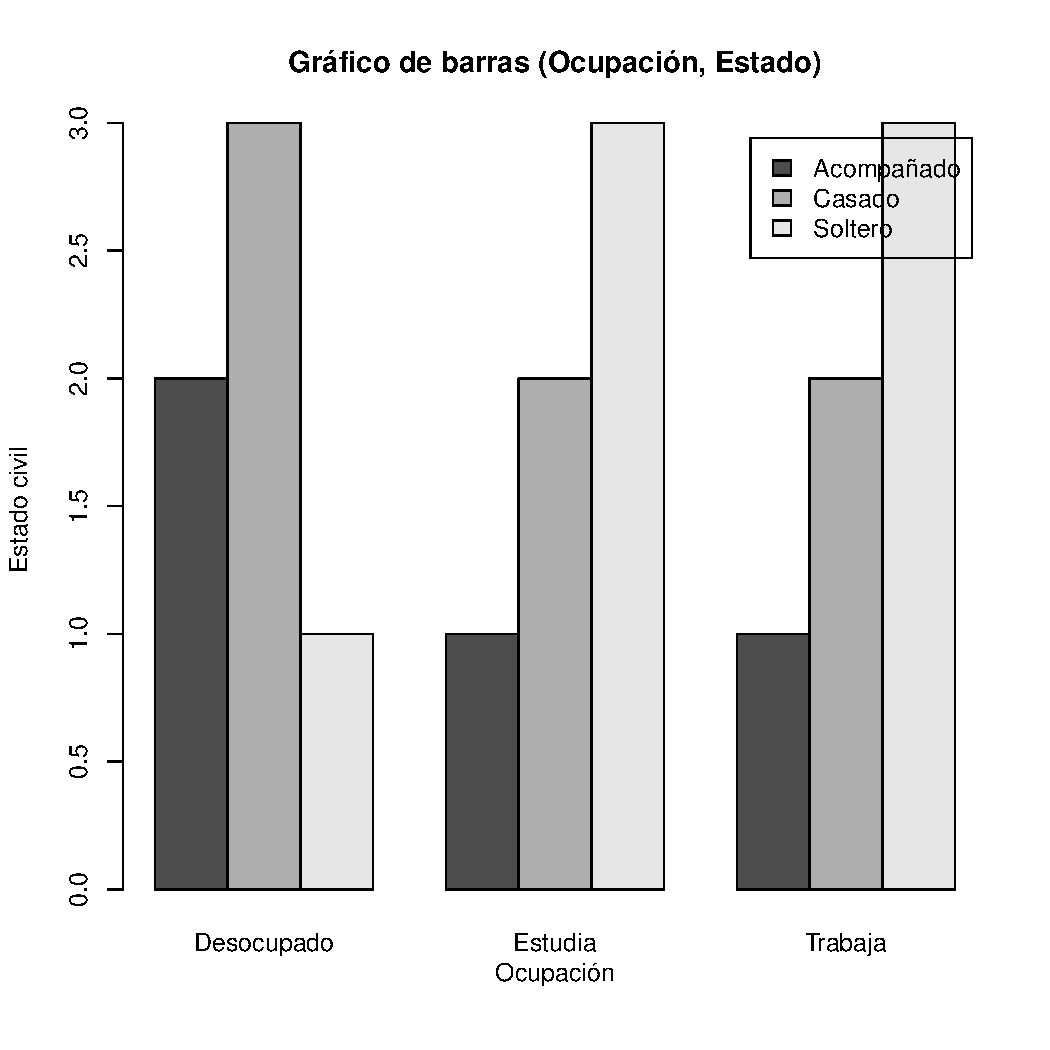
\includegraphics[width=\maxwidth]{figure/unnamed-chunk-1-3} 
\begin{kframe}\begin{alltt}
\hlcom{#Presenta la matriz de covarianzas muestral.}
\hlkwd{options}\hlstd{(}\hlkwc{digits}\hlstd{=}\hlnum{3}\hlstd{)} \hlcom{# s�lo imprime 3 lugares decimales}
\hlstd{S} \hlkwb{<-} \hlkwd{var}\hlstd{(Baterias); S}
\end{alltt}
\begin{verbatim}
##          procesoA procesoB procesoC
## procesoA     11.2     -1.6     12.4
## procesoB     -1.6     14.8     -4.7
## procesoC     12.4     -4.7     20.8
\end{verbatim}
\begin{alltt}
\hlstd{Baterias} \hlkwb{<-} \hlkwd{stack}\hlstd{(Baterias); Baterias}
\end{alltt}
\begin{verbatim}
##    values      ind
## 1     100 procesoA
## 2      96 procesoA
## 3      92 procesoA
## 4      96 procesoA
## 5      92 procesoA
## 6      76 procesoB
## 7      80 procesoB
## 8      75 procesoB
## 9      84 procesoB
## 10     82 procesoB
## 11    108 procesoC
## 12    100 procesoC
## 13     96 procesoC
## 14     98 procesoC
## 15    100 procesoC
\end{verbatim}
\begin{alltt}
\hlkwd{names}\hlstd{(Baterias)} \hlcom{# Muestra los encabezados de los vectores}
\end{alltt}
\begin{verbatim}
## [1] "values" "ind"
\end{verbatim}
\begin{alltt}
\hlkwd{detach}\hlstd{(Baterias,} \hlkwc{pos}\hlstd{=}\hlnum{2}\hlstd{);} \hlkwd{search}\hlstd{()}
\end{alltt}
\begin{verbatim}
##  [1] ".GlobalEnv"        "package:knitr"     "package:stats"    
##  [4] "package:graphics"  "package:grDevices" "package:utils"    
##  [7] "package:datasets"  "package:methods"   "Autoloads"        
## [10] "package:base"
\end{verbatim}
\begin{alltt}
\hlcom{#An�lisis de una variable bidimensional}

\hlstd{Fuma} \hlkwb{=} \hlkwd{c}\hlstd{(}\hlstr{"Si"}\hlstd{,}\hlstr{"No"}\hlstd{,}\hlstr{"No"}\hlstd{,}\hlstr{"Si"}\hlstd{,}\hlstr{"No"}\hlstd{,}\hlstr{"Si"}\hlstd{,}\hlstr{"Si"}\hlstd{,}\hlstr{"Si"}\hlstd{,}\hlstr{"No"}\hlstd{,}\hlstr{"Si"}\hlstd{); Fuma}
\end{alltt}
\begin{verbatim}
##  [1] "Si" "No" "No" "Si" "No" "Si" "Si" "Si" "No" "Si"
\end{verbatim}
\begin{alltt}
\hlstd{Cantidad} \hlkwb{=} \hlkwd{c}\hlstd{(}\hlnum{1}\hlstd{,}\hlnum{2}\hlstd{,}\hlnum{2}\hlstd{,}\hlnum{3}\hlstd{,}\hlnum{3}\hlstd{,}\hlnum{1}\hlstd{,}\hlnum{2}\hlstd{,}\hlnum{1}\hlstd{,}\hlnum{3}\hlstd{,}\hlnum{2}\hlstd{); Cantidad}
\end{alltt}
\begin{verbatim}
##  [1] 1 2 2 3 3 1 2 1 3 2
\end{verbatim}
\begin{alltt}
\hlstd{Estudia} \hlkwb{<-} \hlkwd{data.frame}\hlstd{(}\hlkwc{Fuma}\hlstd{=Fuma,} \hlkwc{Cantidad}\hlstd{=Cantidad); Estudia}
\end{alltt}
\begin{verbatim}
##    Fuma Cantidad
## 1    Si        1
## 2    No        2
## 3    No        2
## 4    Si        3
## 5    No        3
## 6    Si        1
## 7    Si        2
## 8    Si        1
## 9    No        3
## 10   Si        2
\end{verbatim}
\begin{alltt}
\hlkwd{fix}\hlstd{(Estudia)}
\hlkwd{write.table}\hlstd{(Estudia,} \hlkwc{file}\hlstd{=}\hlstr{"Estudia.txt"}\hlstd{,} \hlkwc{append}\hlstd{=}\hlnum{FALSE}\hlstd{,} \hlkwc{quote}\hlstd{=}\hlnum{TRUE}\hlstd{,} \hlkwc{sep}\hlstd{=}\hlstr{" "}\hlstd{,} \hlkwc{na}\hlstd{=}\hlstr{"NA"}\hlstd{,}
\hlkwc{col.names}\hlstd{=}\hlnum{TRUE}\hlstd{)}
\hlstd{write.table}
\end{alltt}
\begin{verbatim}
## function (x, file = "", append = FALSE, quote = TRUE, sep = " ", 
##     eol = "\n", na = "NA", dec = ".", row.names = TRUE, col.names = TRUE, 
##     qmethod = c("escape", "double"), fileEncoding = "") 
## {
##     qmethod <- match.arg(qmethod)
##     if (is.logical(quote) && (length(quote) != 1L || is.na(quote))) 
##         stop("'quote' must be 'TRUE', 'FALSE' or numeric")
##     quoteC <- if (is.logical(quote)) 
##         quote
##     else TRUE
##     qset <- is.logical(quote) && quote
##     if (!is.data.frame(x) && !is.matrix(x)) 
##         x <- data.frame(x)
##     makeRownames <- isTRUE(row.names)
##     makeColnames <- is.logical(col.names) && !identical(FALSE, 
##         col.names)
##     if (is.matrix(x)) {
##         p <- ncol(x)
##         d <- dimnames(x)
##         if (is.null(d)) 
##             d <- list(NULL, NULL)
##         if (is.null(d[[1L]]) && makeRownames) 
##             d[[1L]] <- seq_len(nrow(x))
##         if (is.null(d[[2L]]) && makeColnames && p > 0L) 
##             d[[2L]] <- paste0("V", 1L:p)
##         if (qset) 
##             quote <- if (is.character(x)) 
##                 seq_len(p)
##             else numeric()
##     }
##     else {
##         if (qset) 
##             quote <- if (length(x)) 
##                 which(unlist(lapply(x, function(x) is.character(x) || 
##                   is.factor(x))))
##             else numeric()
##         if (any(sapply(x, function(z) length(dim(z)) == 2 && 
##             dim(z)[2L] > 1))) {
##             c1 <- names(x)
##             x <- as.matrix(x, rownames.force = makeRownames)
##             d <- dimnames(x)
##             if (qset) {
##                 ord <- match(c1, d[[2L]], 0L)
##                 quote <- ord[quote]
##                 quote <- quote[quote > 0L]
##             }
##         }
##         else d <- list(if (makeRownames) row.names(x), if (makeColnames) names(x))
##         p <- ncol(x)
##     }
##     nocols <- p == 0L
##     if (is.logical(quote)) 
##         quote <- NULL
##     else if (is.numeric(quote)) {
##         if (any(quote < 1L | quote > p)) 
##             stop("invalid numbers in 'quote'")
##     }
##     else stop("invalid 'quote' specification")
##     rn <- FALSE
##     rnames <- NULL
##     if (is.logical(row.names)) {
##         if (row.names) {
##             rnames <- as.character(d[[1L]])
##             rn <- TRUE
##         }
##     }
##     else {
##         rnames <- as.character(row.names)
##         rn <- TRUE
##         if (length(rnames) != nrow(x)) 
##             stop("invalid 'row.names' specification")
##     }
##     if (!is.null(quote) && rn) 
##         quote <- c(0, quote)
##     if (is.logical(col.names)) {
##         if (!rn && is.na(col.names)) 
##             stop("'col.names = NA' makes no sense when 'row.names = FALSE'")
##         col.names <- if (is.na(col.names) && rn) 
##             c("", d[[2L]])
##         else if (col.names) 
##             d[[2L]]
##         else NULL
##     }
##     else {
##         col.names <- as.character(col.names)
##         if (length(col.names) != p) 
##             stop("invalid 'col.names' specification")
##     }
##     if (file == "") 
##         file <- stdout()
##     else if (is.character(file)) {
##         file <- if (nzchar(fileEncoding)) 
##             file(file, ifelse(append, "a", "w"), encoding = fileEncoding)
##         else file(file, ifelse(append, "a", "w"))
##         on.exit(close(file))
##     }
##     else if (!isOpen(file, "w")) {
##         open(file, "w")
##         on.exit(close(file))
##     }
##     if (!inherits(file, "connection")) 
##         stop("'file' must be a character string or connection")
##     qstring <- switch(qmethod, escape = "\\\\\"", double = "\"\"")
##     if (!is.null(col.names)) {
##         if (append) 
##             warning("appending column names to file")
##         if (quoteC) 
##             col.names <- paste("\"", gsub("\"", qstring, col.names), 
##                 "\"", sep = "")
##         writeLines(paste(col.names, collapse = sep), file, sep = eol)
##     }
##     if (nrow(x) == 0L) 
##         return(invisible())
##     if (nocols && !rn) 
##         return(cat(rep.int(eol, NROW(x)), file = file, sep = ""))
##     if (is.matrix(x) && !is.atomic(x)) 
##         mode(x) <- "character"
##     if (is.data.frame(x)) {
##         x[] <- lapply(x, function(z) {
##             if (is.object(z) && !is.factor(z)) 
##                 as.character(z)
##             else z
##         })
##     }
##     invisible(.External2(C_writetable, x, file, nrow(x), p, rnames, 
##         sep, eol, na, dec, as.integer(quote), qmethod != "double"))
## }
## <bytecode: 0x000000000b141328>
## <environment: namespace:utils>
\end{verbatim}
\begin{alltt}
\hlkwd{ls}\hlstd{()}
\end{alltt}
\begin{verbatim}
## [1] "Baterias" "Cantidad" "Estudia"  "Fuma"     "S"
\end{verbatim}
\begin{alltt}
\hlkwd{rm}\hlstd{(}\hlkwc{list}\hlstd{=}\hlkwd{ls}\hlstd{(}\hlkwc{all}\hlstd{=}\hlnum{TRUE}\hlstd{))}
\hlkwd{ls}\hlstd{()}
\end{alltt}
\begin{verbatim}
## character(0)
\end{verbatim}
\begin{alltt}
\hlstd{Estudia} \hlkwb{<-} \hlkwd{read.table}\hlstd{(}\hlstr{"Estudia.txt"}\hlstd{,} \hlkwc{header}\hlstd{=}\hlnum{TRUE}\hlstd{)}
\hlstd{Estudia}
\end{alltt}
\begin{verbatim}
##    Fuma Cantidad
## 1    Si        1
## 2    No        2
## 3    No        2
## 4    Si        3
## 5    No        3
## 6    Si        1
## 7    Si        2
## 8    Si        1
## 9    No        3
## 10   Si        2
\end{verbatim}
\begin{alltt}
\hlstd{tablaCont} \hlkwb{<-} \hlkwd{table}\hlstd{(Estudia)}
\hlstd{tablaCont}
\end{alltt}
\begin{verbatim}
##     Cantidad
## Fuma 1 2 3
##   No 0 2 2
##   Si 3 2 1
\end{verbatim}
\begin{alltt}
\hlkwd{options}\hlstd{(}\hlkwc{digits}\hlstd{=}\hlnum{3}\hlstd{)} \hlcom{# s�lo imprime 3 lugares decimales}
\hlstd{propTotal} \hlkwb{<-} \hlkwd{prop.table}\hlstd{(tablaCont); propTotal}
\end{alltt}
\begin{verbatim}
##     Cantidad
## Fuma   1   2   3
##   No 0.0 0.2 0.2
##   Si 0.3 0.2 0.1
\end{verbatim}
\begin{alltt}
\hlstd{propFila} \hlkwb{<-} \hlkwd{prop.table}\hlstd{(tablaCont,} \hlnum{1}\hlstd{)}
\hlstd{propFila}
\end{alltt}
\begin{verbatim}
##     Cantidad
## Fuma     1     2     3
##   No 0.000 0.500 0.500
##   Si 0.500 0.333 0.167
\end{verbatim}
\begin{alltt}
\hlstd{propCol} \hlkwb{<-} \hlkwd{prop.table}\hlstd{(tablaCont,} \hlnum{2}\hlstd{)}
\hlstd{propCol}
\end{alltt}
\begin{verbatim}
##     Cantidad
## Fuma     1     2     3
##   No 0.000 0.500 0.667
##   Si 1.000 0.500 0.333
\end{verbatim}
\begin{alltt}
\hlkwd{barplot}\hlstd{(}\hlkwd{table}\hlstd{(Estudia}\hlopt{$}\hlstd{Cantidad, Estudia}\hlopt{$}\hlstd{Fuma),} \hlkwc{beside} \hlstd{=} \hlnum{FALSE}\hlstd{,} \hlkwc{horizontal}\hlstd{=}\hlnum{FALSE}\hlstd{,} \hlkwc{main}\hlstd{=}\hlstr{"Gr�fico de barras (Fuma, Cantidad de horas de estudio)"}\hlstd{,} \hlkwc{legend.text} \hlstd{=T,} \hlkwc{xlab}\hlstd{=}\hlstr{"Fuma"}\hlstd{,} \hlkwc{ylab}\hlstd{=}\hlstr{"Cantidad de horas-estudio"}\hlstd{)}
\end{alltt}


{\ttfamily\noindent\color{warningcolor}{\#\# Warning in plot.window(xlim, ylim, log = log, ...): "{}horizontal"{} is not a graphical parameter}}

{\ttfamily\noindent\color{warningcolor}{\#\# Warning in axis(if (horiz) 2 else 1, at = at.l, labels = names.arg, lty = axis.lty, : "{}horizontal"{} is not a graphical parameter}}

{\ttfamily\noindent\color{warningcolor}{\#\# Warning in title(main = main, sub = sub, xlab = xlab, ylab = ylab, ...): "{}horizontal"{} is not a graphical parameter}}

{\ttfamily\noindent\color{warningcolor}{\#\# Warning in axis(if (horiz) 1 else 2, cex.axis = cex.axis, ...): "{}horizontal"{} is not a graphical parameter}}\end{kframe}
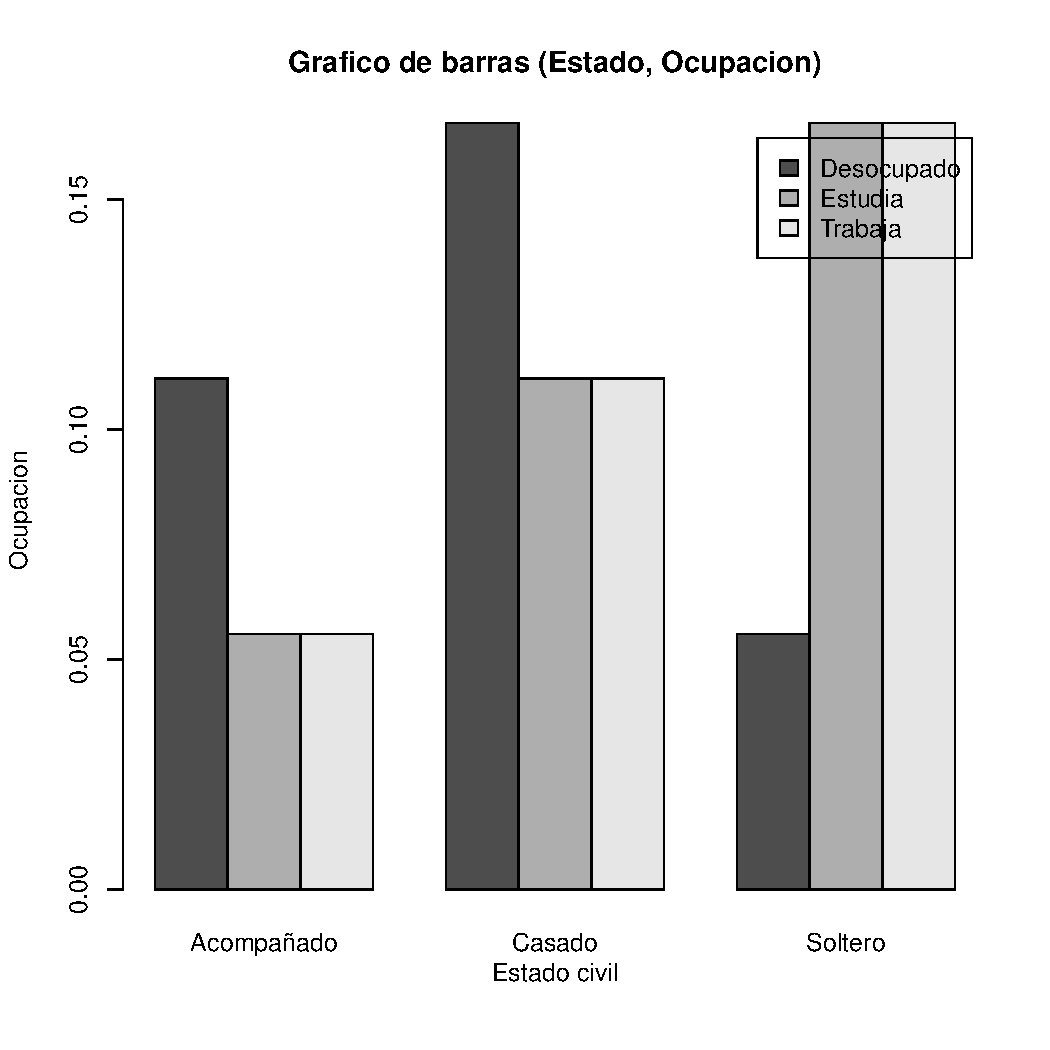
\includegraphics[width=\maxwidth]{figure/unnamed-chunk-1-4} 
\begin{kframe}\begin{alltt}
\hlkwd{barplot}\hlstd{(}\hlkwd{table}\hlstd{(Estudia}\hlopt{$}\hlstd{Fuma, Estudia}\hlopt{$}\hlstd{Cantidad),} \hlkwc{beside} \hlstd{=} \hlnum{FALSE}\hlstd{,} \hlkwc{horizontal}\hlstd{=}\hlnum{FALSE}\hlstd{,}\hlkwc{main}\hlstd{=}\hlstr{"Gr�fico
de barras (Cantidad de horas de estudio,Fuma)"}\hlstd{,} \hlkwc{legend.text} \hlstd{=T,} \hlkwc{xlab}\hlstd{=}\hlstr{"Cantidad de horas-estudio"}\hlstd{,}
\hlkwc{ylab}\hlstd{=}\hlstr{"Fuma"}\hlstd{)}
\end{alltt}


{\ttfamily\noindent\color{warningcolor}{\#\# Warning in plot.window(xlim, ylim, log = log, ...): "{}horizontal"{} is not a graphical parameter}}

{\ttfamily\noindent\color{warningcolor}{\#\# Warning in axis(if (horiz) 2 else 1, at = at.l, labels = names.arg, lty = axis.lty, : "{}horizontal"{} is not a graphical parameter}}

{\ttfamily\noindent\color{warningcolor}{\#\# Warning in title(main = main, sub = sub, xlab = xlab, ylab = ylab, ...): "{}horizontal"{} is not a graphical parameter}}

{\ttfamily\noindent\color{warningcolor}{\#\# Warning in axis(if (horiz) 1 else 2, cex.axis = cex.axis, ...): "{}horizontal"{} is not a graphical parameter}}\end{kframe}
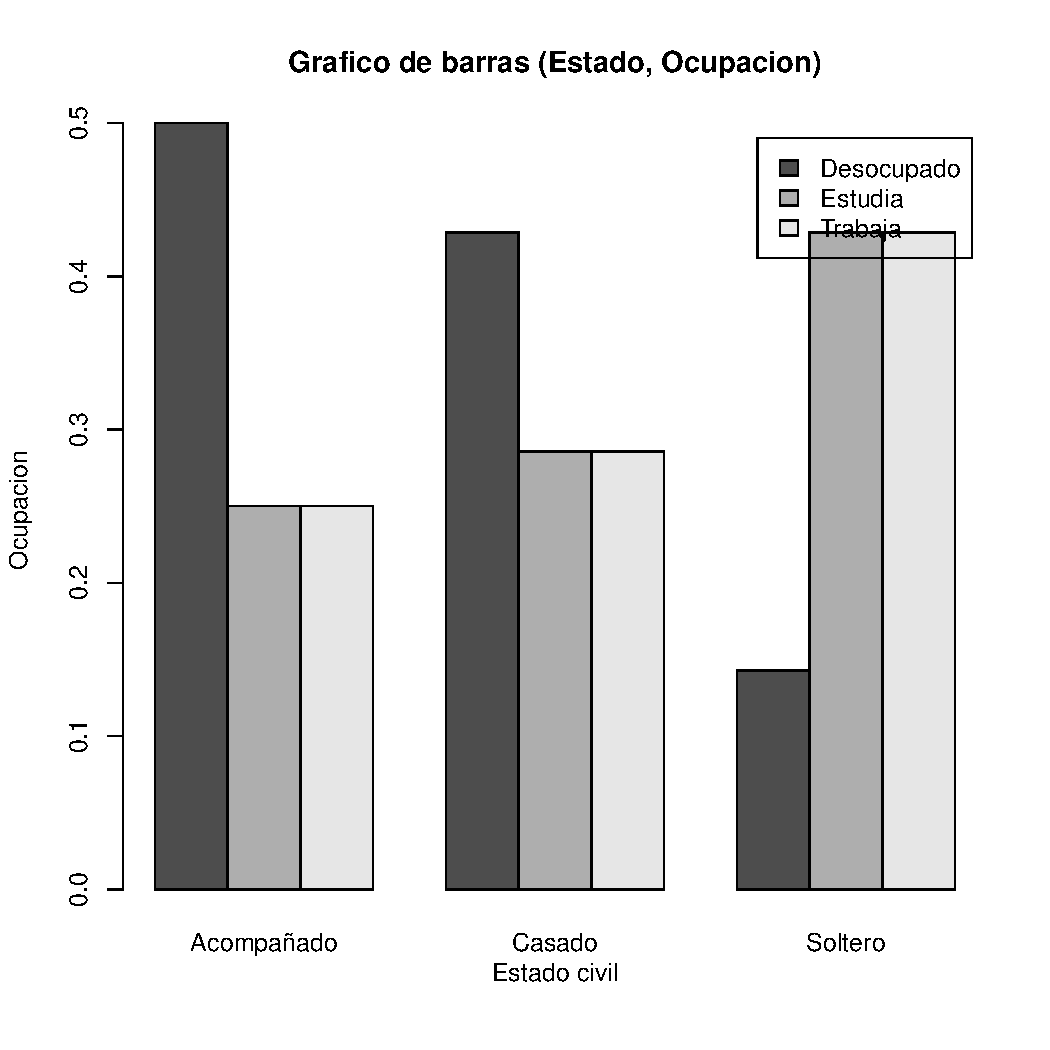
\includegraphics[width=\maxwidth]{figure/unnamed-chunk-1-5} 
\begin{kframe}\begin{alltt}
\hlstd{Fuma}\hlkwb{=}\hlkwd{factor}\hlstd{(Estudia}\hlopt{$}\hlstd{Fuma); Fuma}
\end{alltt}
\begin{verbatim}
##  [1] Si No No Si No Si Si Si No Si
## Levels: No Si
\end{verbatim}
\begin{alltt}
\hlkwd{barplot}\hlstd{(}\hlkwd{table}\hlstd{(Estudia}\hlopt{$}\hlstd{Cantidad, Estudia}\hlopt{$}\hlstd{Fuma),} \hlkwc{main}\hlstd{=}\hlstr{"Gr�fico de barras (Fuma, Cantidad de horas
de estudio)"}\hlstd{,} \hlkwc{xlab}\hlstd{=}\hlstr{"Fuma"}\hlstd{,} \hlkwc{ylab}\hlstd{=}\hlstr{"Cantidad de horas-estudio"}\hlstd{,} \hlkwc{beside}\hlstd{=}\hlnum{TRUE}\hlstd{,} \hlkwc{legend.text}\hlstd{=T)}
\end{alltt}
\end{kframe}
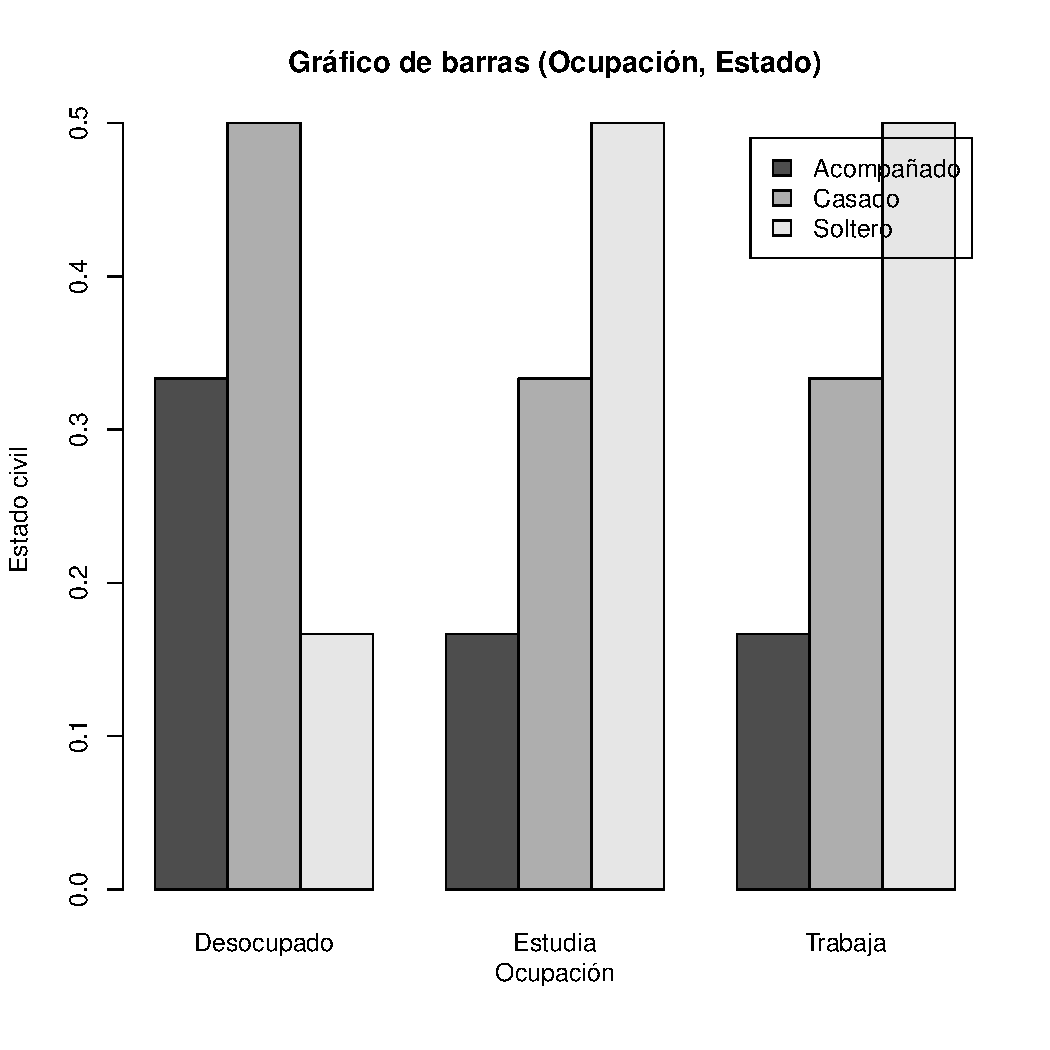
\includegraphics[width=\maxwidth]{figure/unnamed-chunk-1-6} 
\begin{kframe}\begin{alltt}
\hlkwd{barplot}\hlstd{(}\hlkwd{table}\hlstd{(Estudia}\hlopt{$}\hlstd{Cantidad, Estudia}\hlopt{$}\hlstd{Fuma),} \hlkwc{main}\hlstd{=}\hlstr{"Gr�fico de barras (Fuma, Cantidad de horas
de estudio)"}\hlstd{,} \hlkwc{xlab}\hlstd{=}\hlstr{"Fuma"}\hlstd{,} \hlkwc{ylab}\hlstd{=}\hlstr{"Cantidad de horas-estudio"}\hlstd{,} \hlkwc{beside}\hlstd{=}\hlnum{TRUE}\hlstd{,} \hlkwc{legend.text}\hlstd{=}\hlkwd{c}\hlstd{(}\hlstr{"menor
que 5"}\hlstd{,} \hlstr{"5-10"}\hlstd{,} \hlstr{"mayor que 10"}\hlstd{))}
\end{alltt}
\end{kframe}
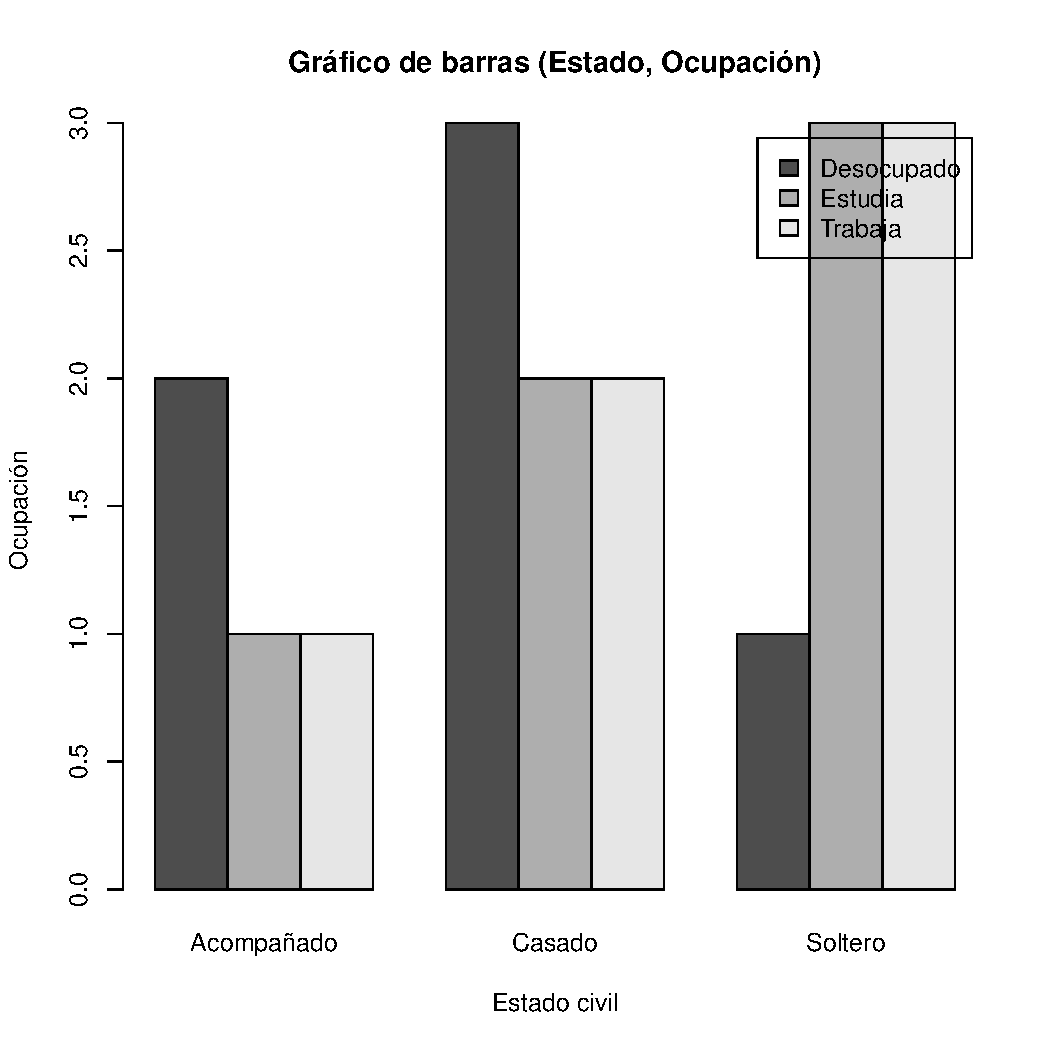
\includegraphics[width=\maxwidth]{figure/unnamed-chunk-1-7} 
\begin{kframe}\begin{alltt}
\hlkwd{chisq.test}\hlstd{(tablaCont)}
\end{alltt}


{\ttfamily\noindent\color{warningcolor}{\#\# Warning in chisq.test(tablaCont): Chi-squared approximation may be incorrect}}\begin{verbatim}
## 
## 	Pearson's Chi-squared test
## 
## data:  tablaCont
## X-squared = 3, df = 2, p-value = 0.2
\end{verbatim}
\begin{alltt}
\hlcom{#Como p-valor es mayor que 0.05, se concluye}
\hlcom{#que las variables con independientes}
\end{alltt}
\end{kframe}
\end{knitrout}



\end{document}
